\makeatletter
\makeatother
\documentclass[10pt,english]{article}\usepackage{graphicx, color}
%% maxwidth is the original width if it is less than linewidth
%% otherwise use linewidth (to make sure the graphics do not exceed the margin)
\usepackage{alltt}
\usepackage[T1]{fontenc}
\usepackage[latin9]{inputenc}
\usepackage{geometry}
\geometry{left=1.5cm,right=1.5cm,top=2cm,bottom=2cm}
\usepackage{fancyhdr}
\pagestyle{fancy}
\setlength{\parskip}{\smallskipamount}
\setlength{\parindent}{0pt}
\usepackage{amsthm}
\usepackage{amsmath}
\usepackage{subfigure}

\makeatletter

%%%%%%%%%%%%%%%%%%%%%%%%%%%%%% LyX specific LaTeX commands.
\providecommand{\LyX}{L\kern-.1667em\lower.25em\hbox{Y}\kern-.125emX\@}

%%%%%%%%%%%%%%%%%%%%%%%%%%%%%% Textclass specific LaTeX commands.
\numberwithin{equation}{section}
\numberwithin{figure}{section}

\@ifundefined{date}{}{\date{}}
%%%%%%%%%%%%%%%%%%%%%%%%%%%%%% User specified LaTeX commands.
\pagestyle{empty} 

\makeatother

\usepackage{babel}
\begin{document}

\title{Week6 Report}


\author{Xiaohui Li, Yuxin Ma}

\maketitle

This week we make the further discussion towards the high-dimensional situation. Firstly, we keep the $\epsilon$ fixed to see the relationship between $N$ and power. Then, we check the scaling behavior of $Y_{max}$ in $\epsilon$ under the dense alternative. Finally, we generate the plots of $\epsilon$ versus $K$. 

\section{Relationship between $N$ and power}
Firstly, we check the relationship between $N$ and power where we control $N$ to increase from 1000 to 100,000. Also, we do the repetitive test for minimum, median and mean statistics for p\_combined value.\\
\begin{figure}[htbp]
\centering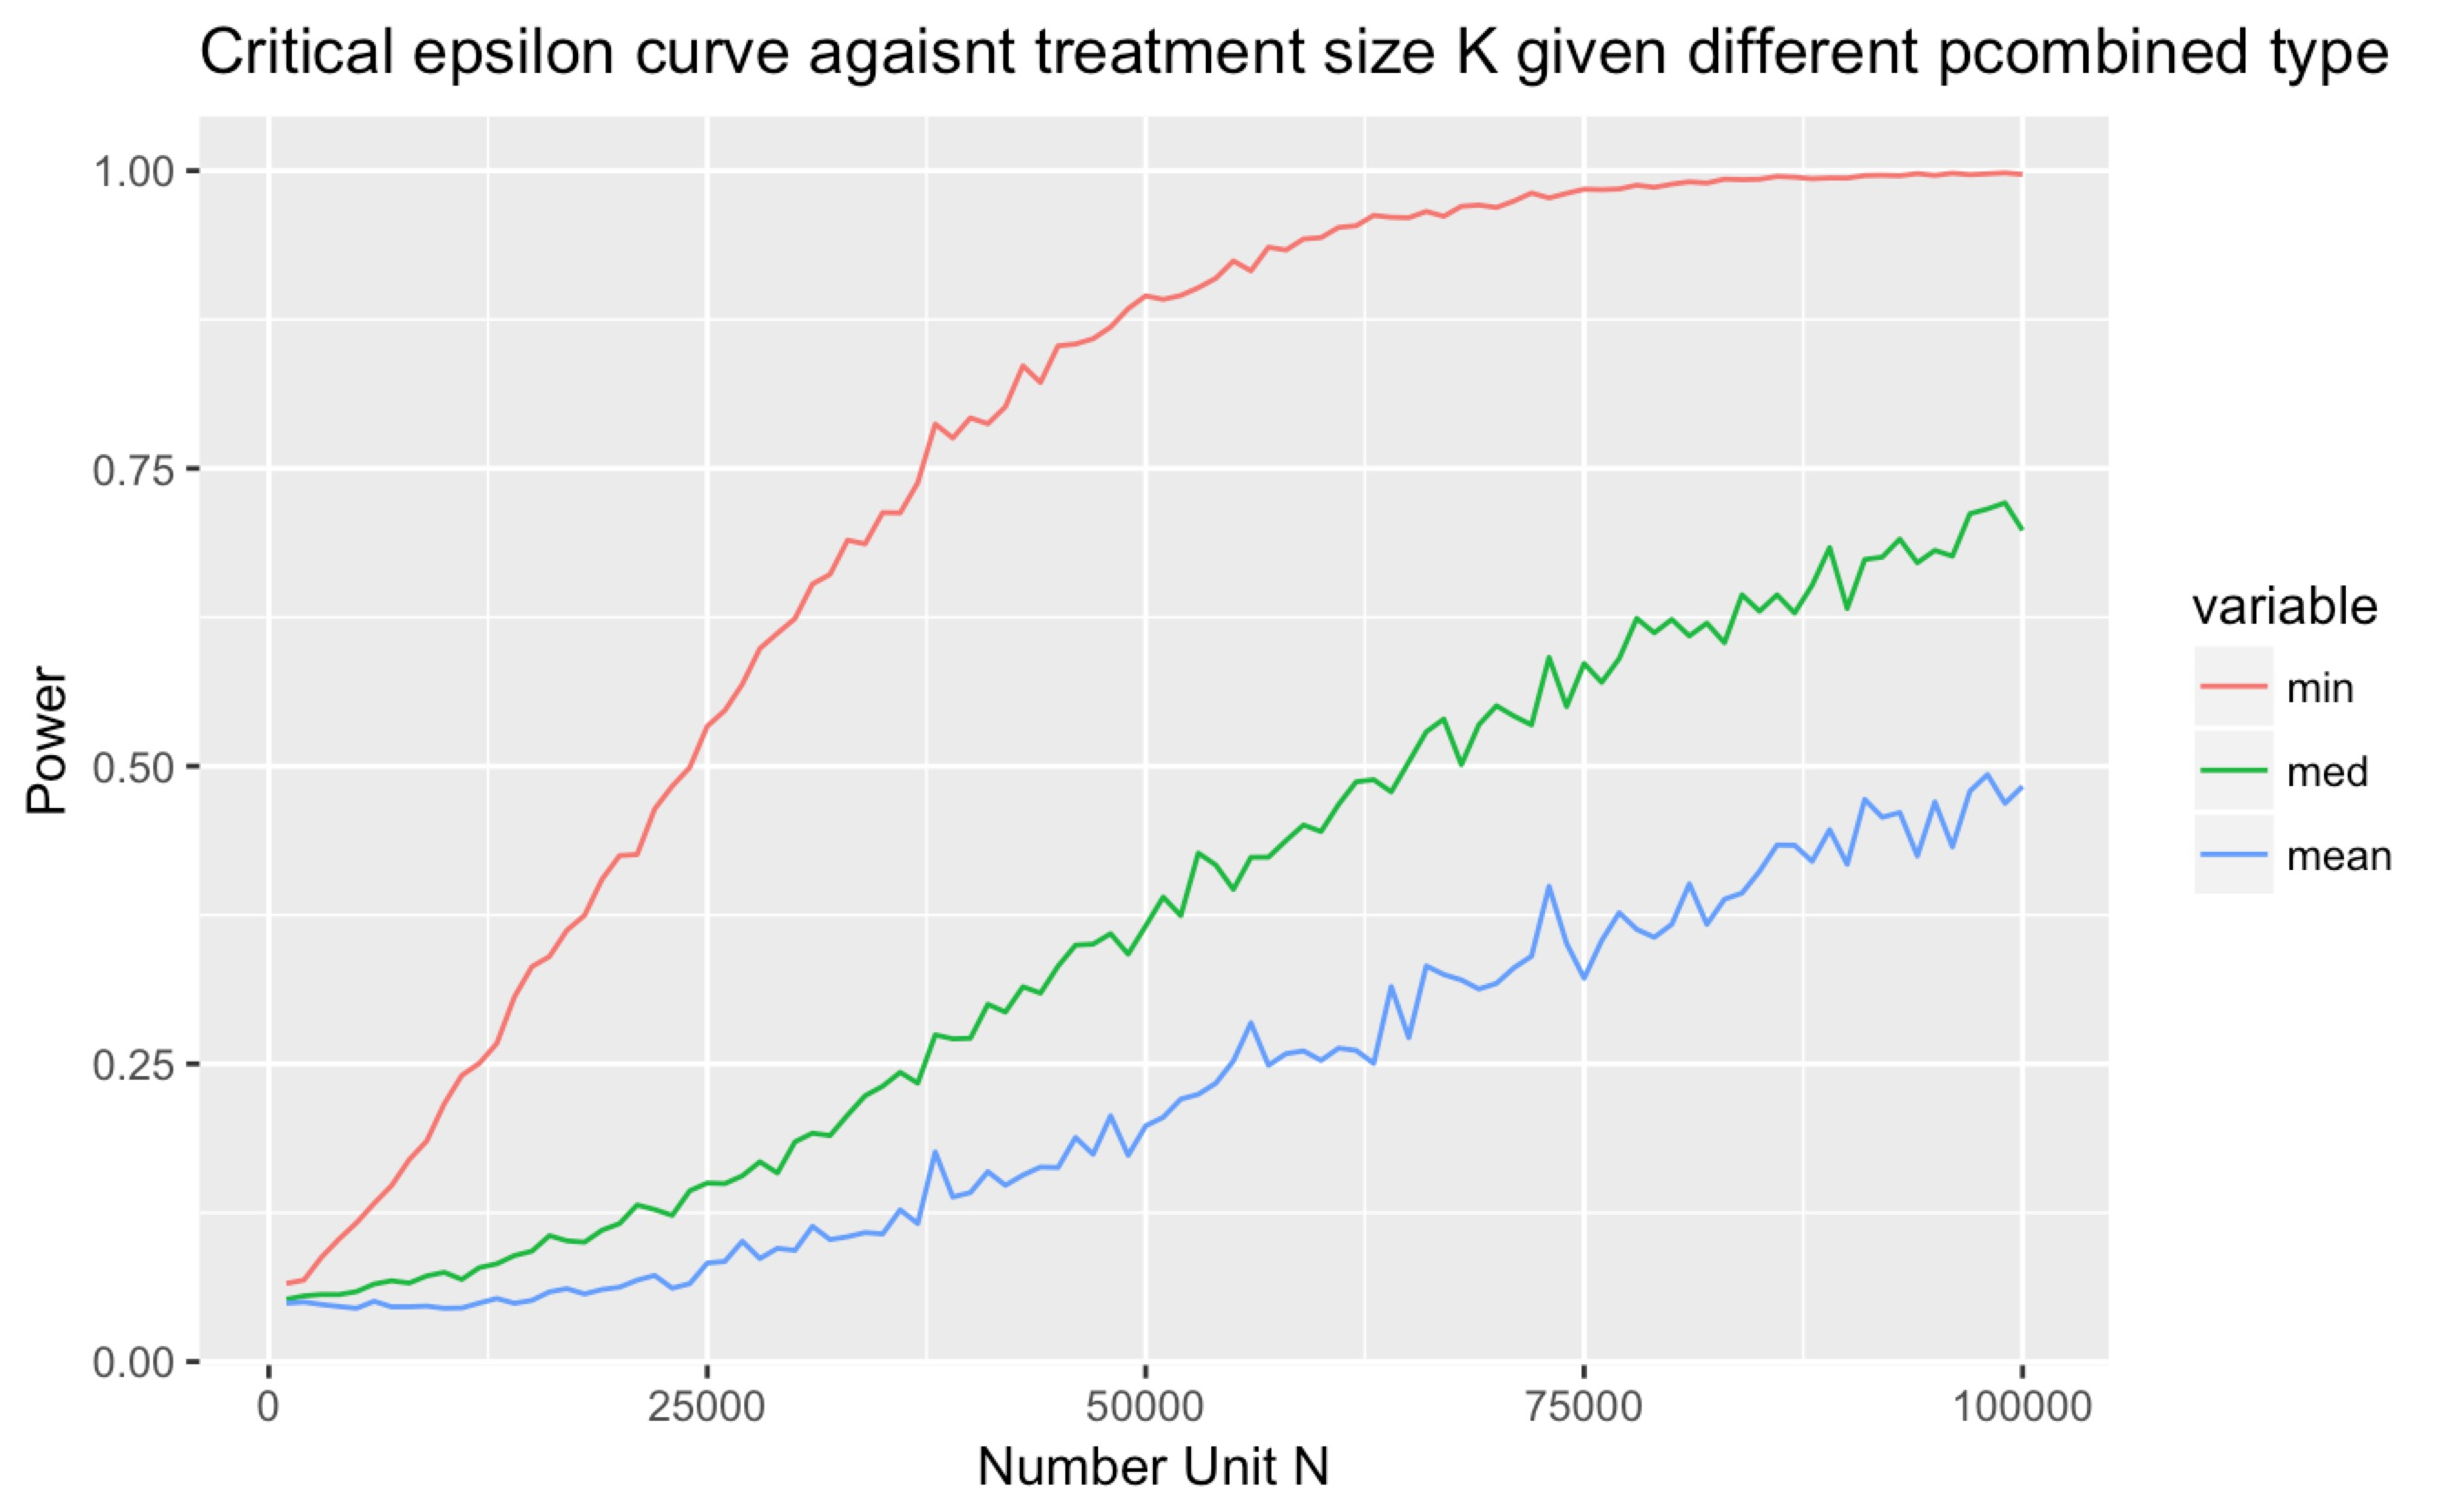
\includegraphics[width=6in, height=4in]{N}
\caption{Relationship between $N$ and power}
\end{figure}
\quad\\
We can see that as $N$ increases, the power will increase as well. And also, the minimum statistics, the black curve, performs best while the median and mean (blue and green ones) do not behave such well.

\section{Scaling behavior of $Y_{max}$}
Next, we check the scaling behavior of $Y_{max}$ in $\epsilon$ under the dense alternative. Since last week we found that for the minimum p\_combined, the critical epsilon of $K$ is a linear curve, and the minimum p\_combined corresponds to the maximum of $Y$, this week we do the scaling behavior of $Y_{max}$ to check whether $Y_{max}$ fits in the $\sqrt{K}$ trend and then makes the critical epsilon curve linear under the minimum p\_combined.\\
\begin{figure}[htbp]
\centering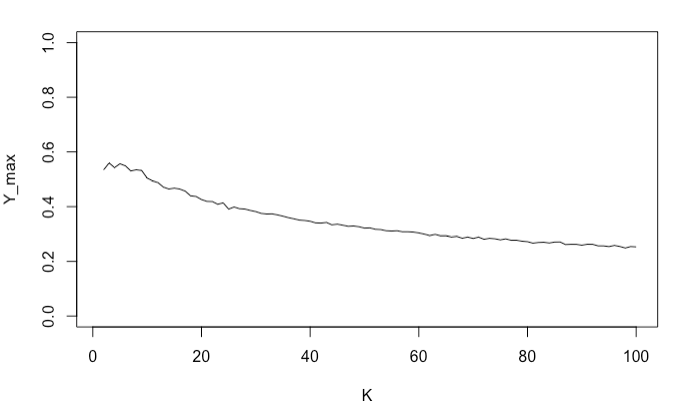
\includegraphics[width=4.5in, height=3in]{max}
\caption{$Y_{max}$ versus $K$}
\end{figure}
\quad\\
Theoretically, We think that it should fit the $\epsilon/\sqrt{K}$ trend and as we take value 1 for the $\epsilon$, $Y_{max}$ should fit $1/\sqrt{K}$. But the result does not look like that. No coefficients for $1/\sqrt{K}$ and $R^2$ equals to 0.\\
\begin{figure}[htbp]
\centering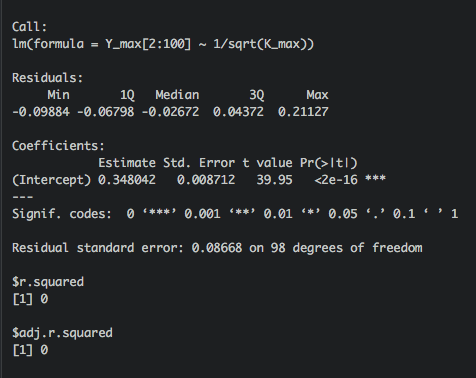
\includegraphics[width=4in, height=3in]{sqrt}
\caption{Fit $1/\sqrt{K}$ to $Y_{max}$}
\end{figure}
\quad\\
Meanwhile, we try other form of $K$ to fit the $Y_{max}$, including $\sqrt{K}$, $1/K$ and $\ln{K}$ etc., and finally we find that $\ln{K}$ has a significant fitting to the $Y_{max}$ where the coefficient is minus and the $R^2$ equals to around 0.96.\\
\begin{figure}[htbp]
\centering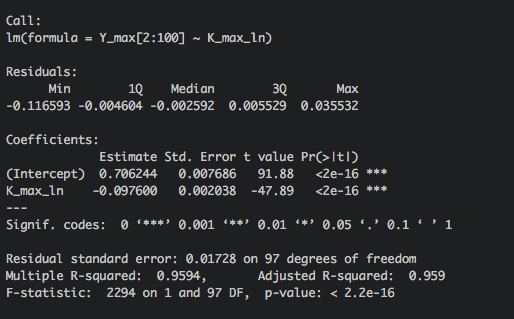
\includegraphics[width=4in, height=3in]{ln}
\caption{Fit $\ln{K}$ to $Y_{max}$}
\end{figure}
\quad\\
\quad\\
\quad\\
\quad\\
\quad\\
\quad\\
It is not expected according to our intuition, so the result is really surprising. Theoretically, we need $Y_{max}$ to fit $1/\sqrt{K}$ to keep the critical $\epsilon$ to be linear for the minimum p\_combined, but the result contradicts with that. Maybe there exists other explanations.

\section{Critical $\epsilon$ for $K$}
Last week we check the critical $\epsilon$ for $K$ as the p\_combined take the minimum statistics. This week for further discussion, we also take the median and mean statistics for p\_combined to check their trends.\\
\begin{figure}[htbp]
\centering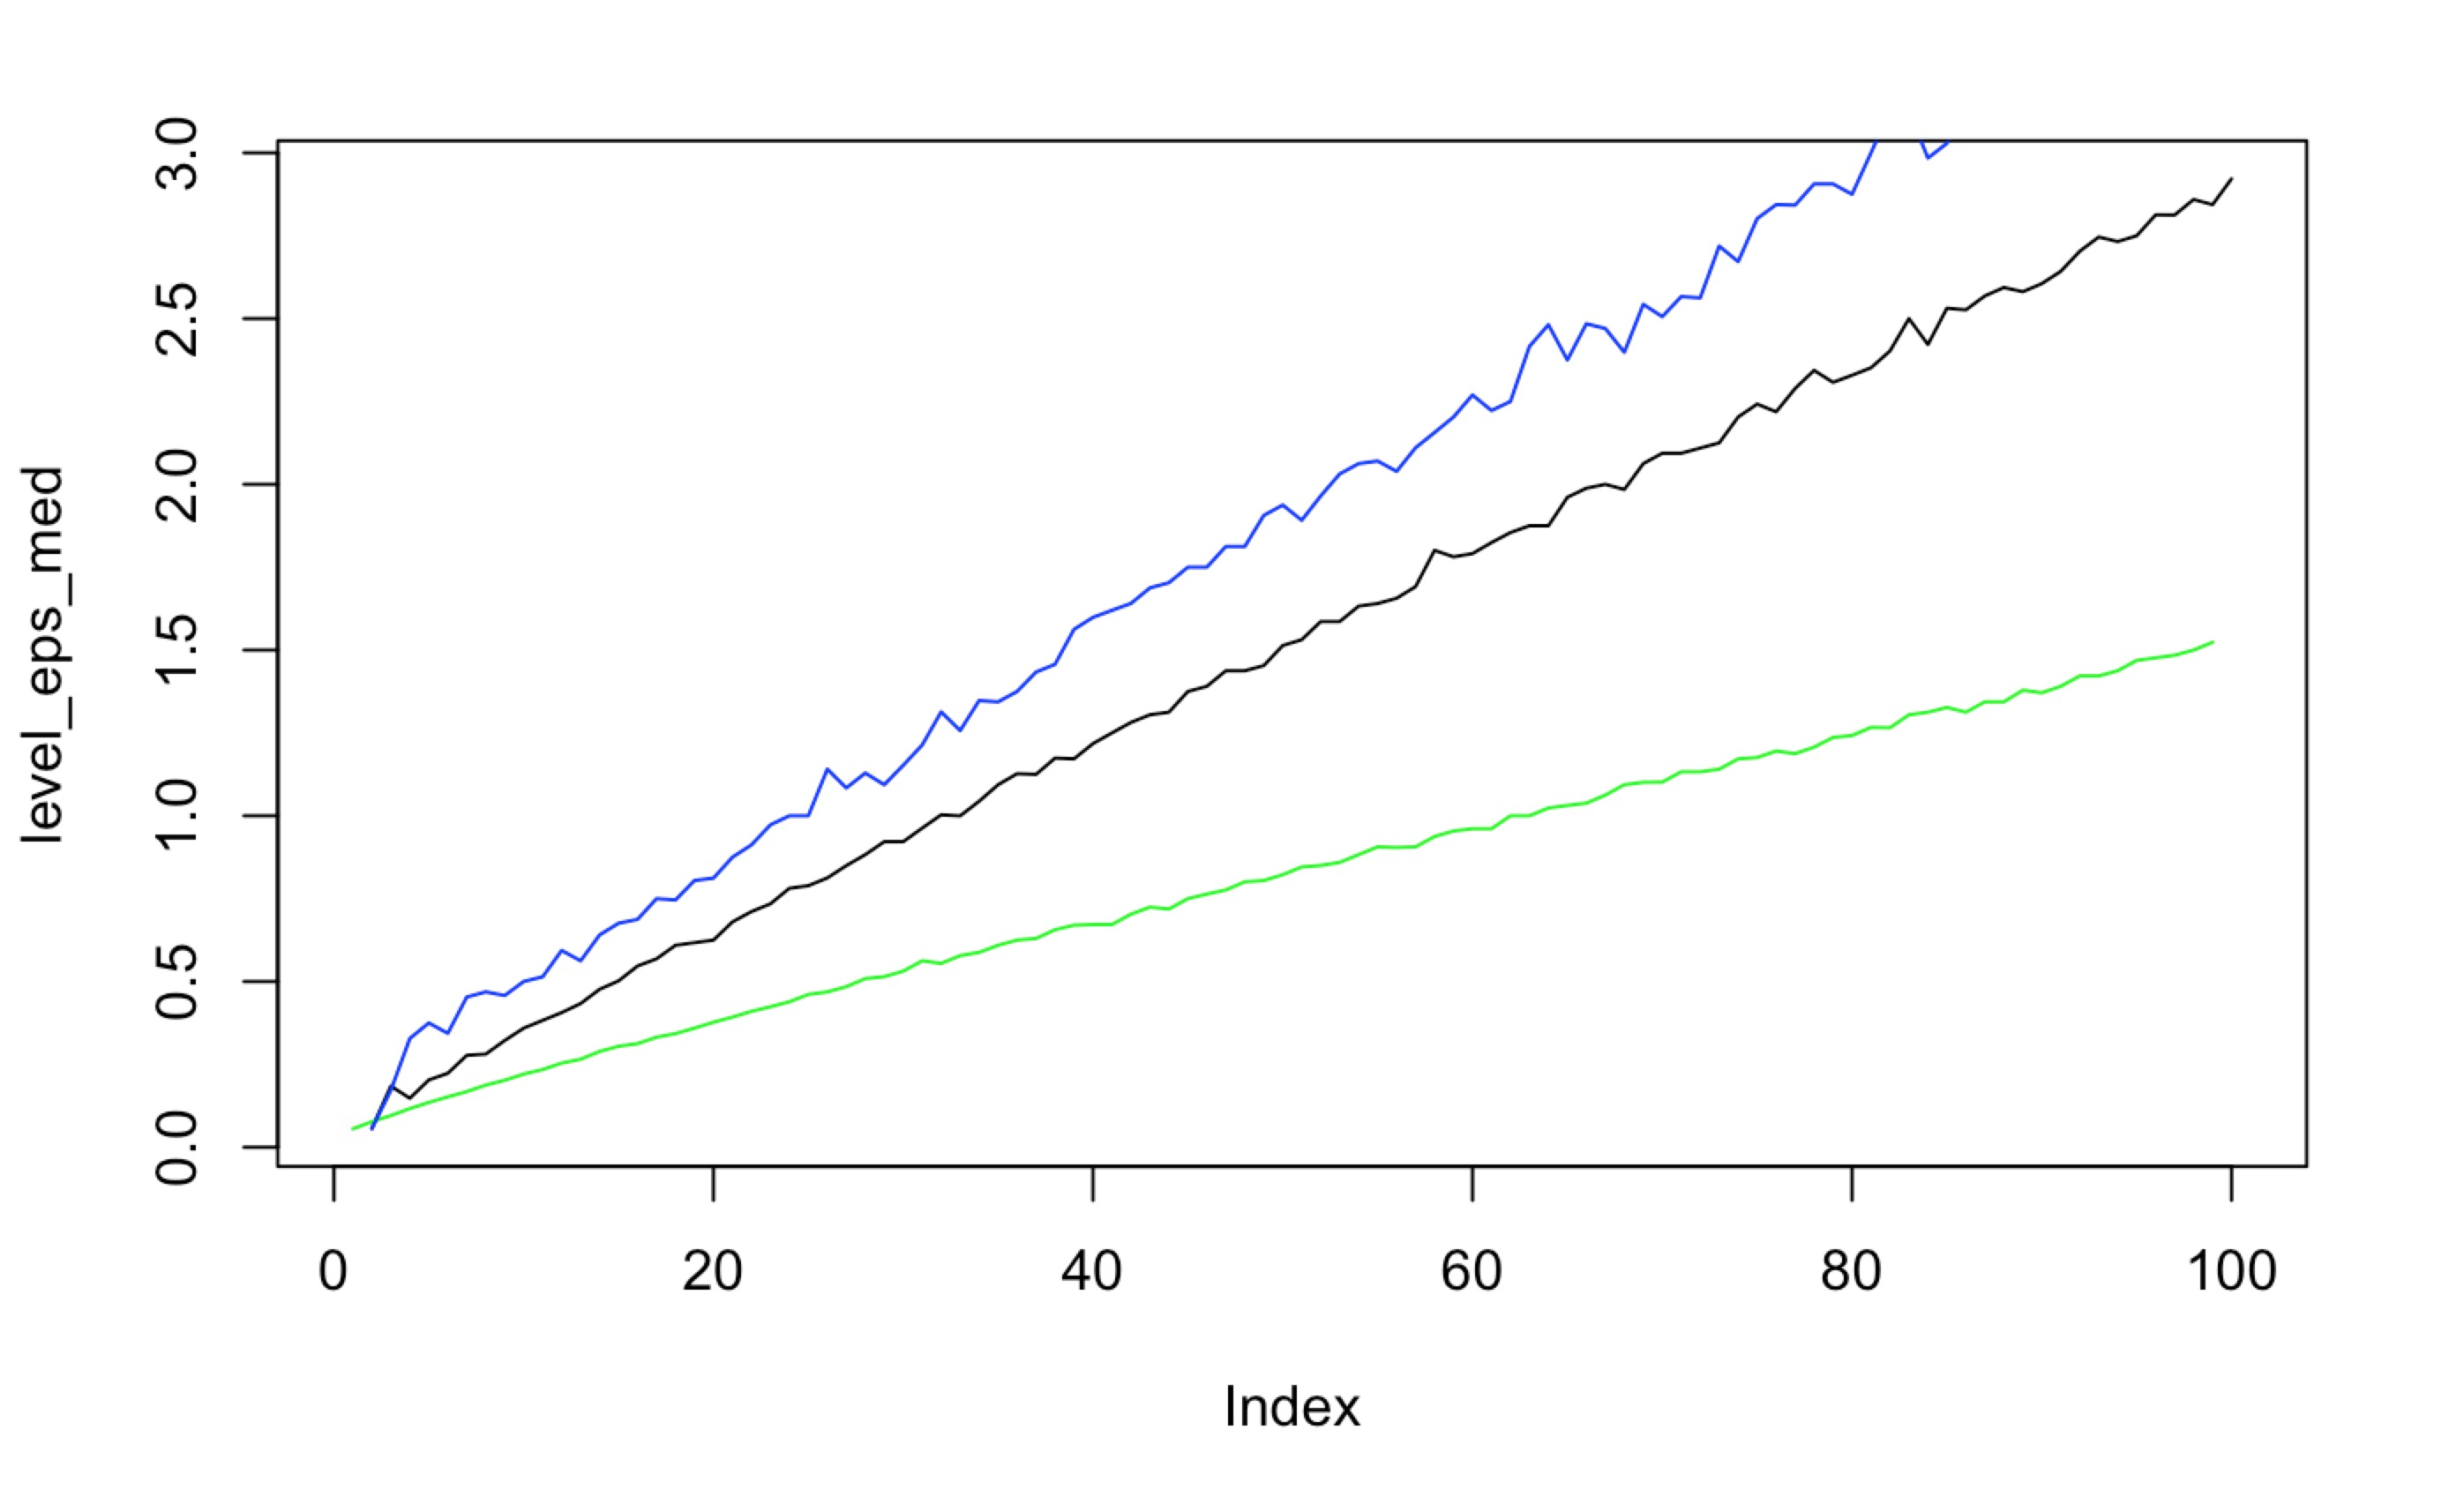
\includegraphics[width=5in, height=3.4in]{cr}
\caption{Critical $\epsilon$ for $K$}
\end{figure}
\quad\\
\quad\\
We can see that all three curves, green to the minimum, black to the median, blue to the mean, follow an obvious linear trend and the minimum is the lowest curve, which corresponds to our intuition. And also we can notice that as $K$ increases, the mean and median become unstable to some degrees.\\
\quad\\
But it is interesting that all of them follow the linear trend, which means that only $Y_{max}$ probably cannot explain all of them. Meanwhile, from last part, we can see that the fitting result of $Y_{max}$ and $1/\sqrt{K}$ considering minimum p\_combined also contradicts to our assumption. So maybe we need further discussion to the critical $\epsilon$.


\end{document}










